\documentclass{standalone}
\usepackage{tikz}
\usetikzlibrary{mindmap}

\begin{document}

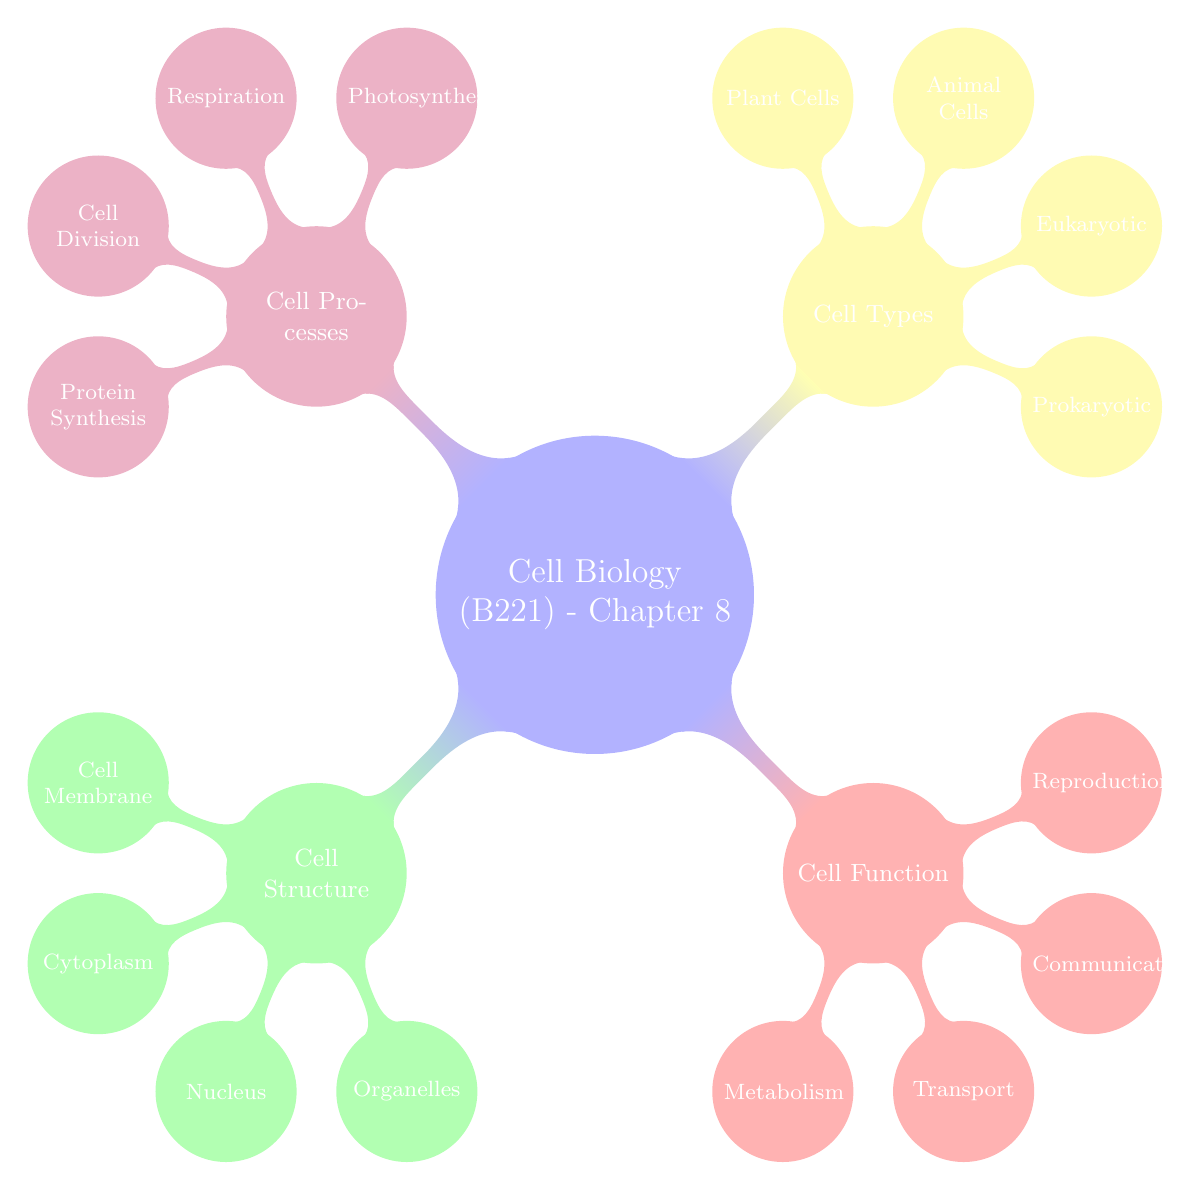
\begin{tikzpicture}[mindmap, grow cyclic, every node/.style=concept, concept color=blue!30, text=white, level 1/.append style={level distance=5cm,sibling angle=90}, level 2/.append style={level distance=3cm,sibling angle=45}]
  \node[concept] {Cell Biology (B221) - Chapter 8}
    child [concept color=green!30] { node {Cell Structure}
      child { node {Cell Membrane} }
      child { node {Cytoplasm} }
      child { node {Nucleus} }
      child { node {Organelles} }
    }
    child [concept color=red!30] { node {Cell Function}
      child { node {Metabolism} }
      child { node {Transport} }
      child { node {Communication} }
      child { node {Reproduction} }
    }
    child [concept color=yellow!30] { node {Cell Types}
      child { node {Prokaryotic} }
      child { node {Eukaryotic} }
      child { node {Animal Cells} }
      child { node {Plant Cells} }
    }
    child [concept color=purple!30] { node {Cell Processes}
      child { node {Photosynthesis} }
      child { node {Respiration} }
      child { node {Cell Division} }
      child { node {Protein Synthesis} }
    };
\end{tikzpicture}

\end{document}